%
% ---------- header -----------------------------------------------------------
%
% project       kaneton
%
% license       kaneton
%
% file          /home/mycure/kaneton/view/book/kaneton/design.tex
%
% created       julien quintard   [mon dec 17 12:26:46 2007]
% updated       julien quintard   [mon dec 17 15:21:40 2007]
%

%
% ---------- design -----------------------------------------------------------
%

\chapter{Design}
\label{chapter:design}

This chapter introduces the kaneton design and its very specific terminology.

\newpage

%
% ---------- text -------------------------------------------------------------
%

%
% managers
%

\section{Managers}

Although microkernel-based operating systems are, by nature, modular, kaneton
people wanted the microkernel itself to be modular, subdivided into logical
parts. This subdivision was introduced to make the whole microkernel clearer
and more understandable.

The kaneton microkernel is thus divided into \textbf{managers}. These
managers are generally responsible for a \textbf{kaneton object} type but there
exist managers which manage something else or just create an abstraction over
other kaneton managers. A kaneton object represents a logical and fundamental
kernel entity. These objects are described later in this section.

\textit{Figure \ref{figure:managers-organisation}} illustrates the
decomposition of the microkernel into multiples managers.

\begin{figure}[h]
  \begin{center}
    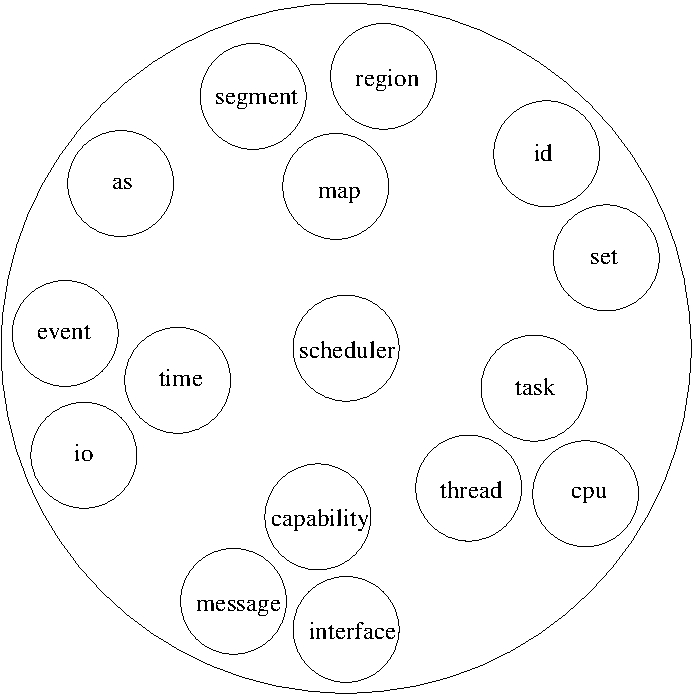
\includegraphics[scale=0.7]{\path/figures/managers-organisation.pdf}
    \caption{kaneton managers.}
    \label{figure:managers-organisation}
  \end{center}
\end{figure}

Note that this decomposition has no direct relation with the \textit{Object
Programming} paradigm. Indeed, even if kaneton designers tried to reduce the
dependencies between the managers, some managers remain intrusive as they
access the data structures of one or more other managers.

A kaneton object represents a kernel entity. Every object is identified by
an unique identifier issued and managed by the \textbf{id} manager.

kaneton people believe a kernel is composed of data structures and processing,
each of these should be very clearly dissociated. The \textbf{set} manager is
heavily used by the other kaneton managers for storing data without taking
care of how it is technically done. The set concept was introduced to make
the microkernel code as clear as pseudo code.

\textit{Figure \ref{figure:sets-organisation}} depicts the set manager
composed of a set container which holds descriptor of the actual data
structures.

\begin{figure}[h]
  \begin{center}
    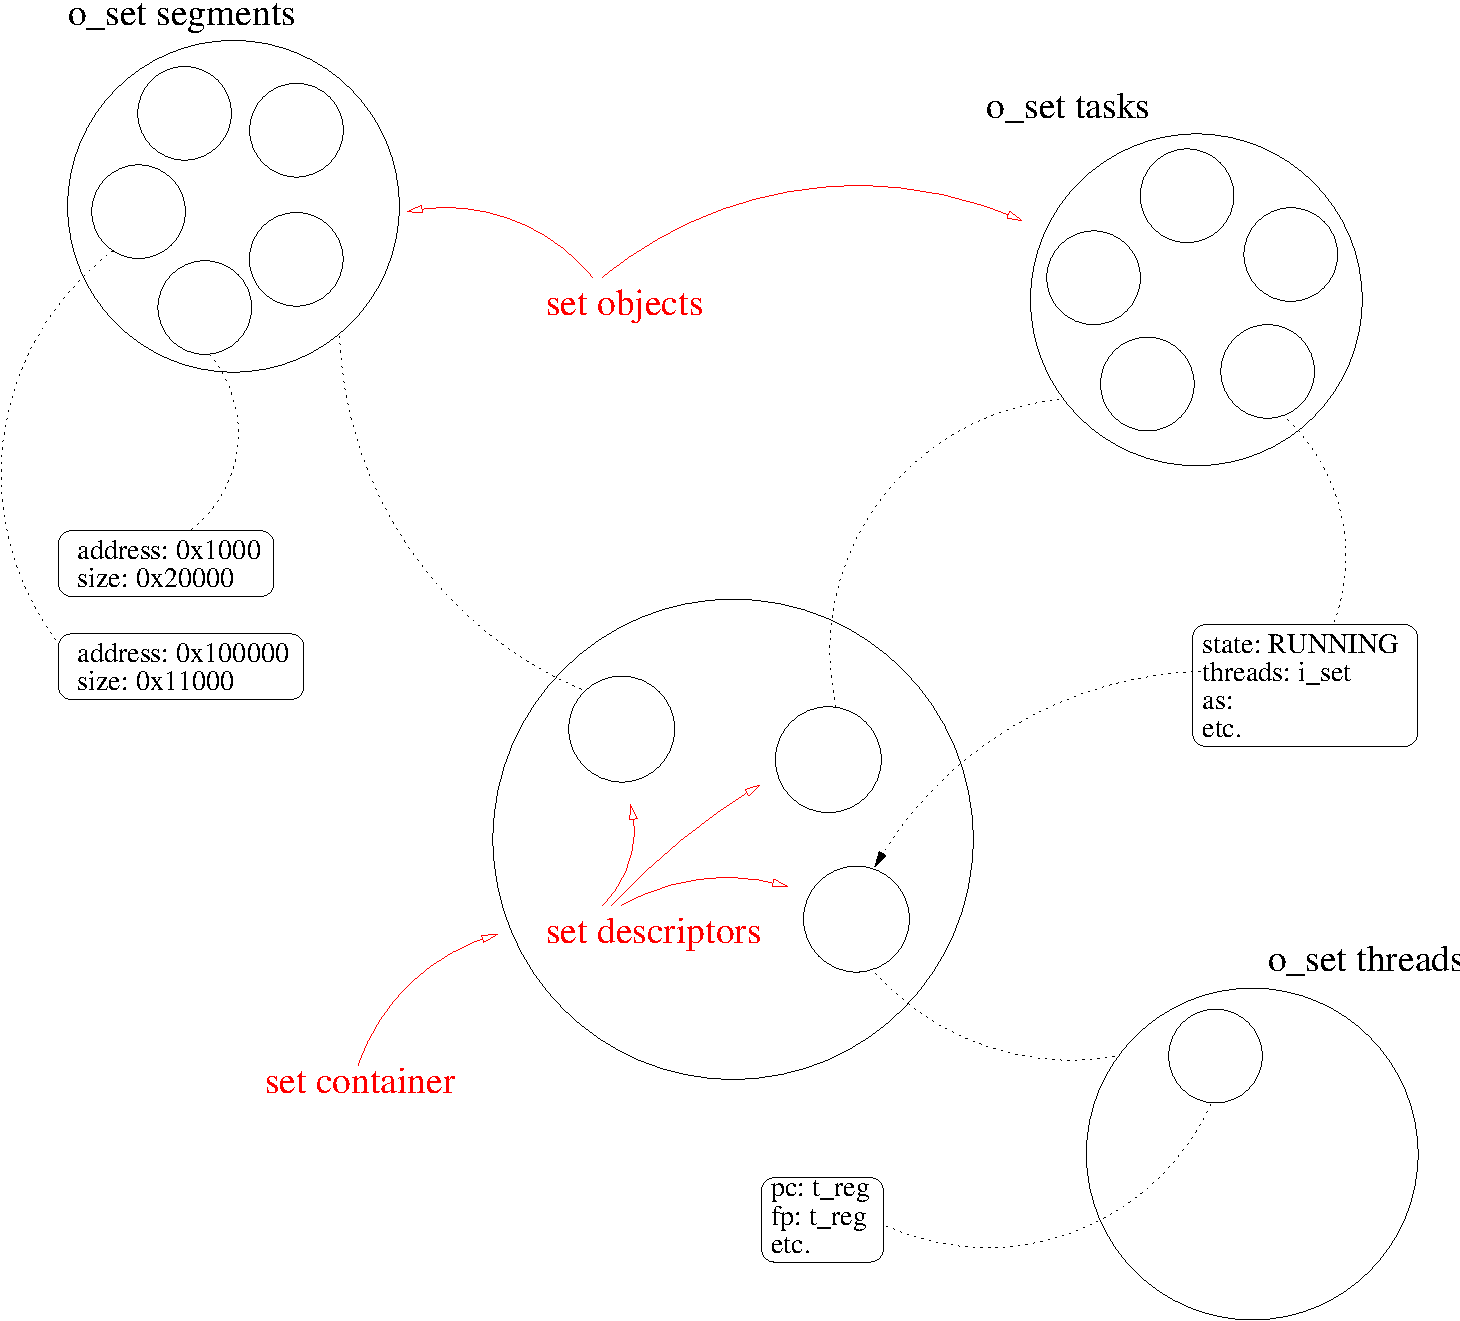
\includegraphics[scale=0.5]{\path/figures/sets-organisation.pdf}
    \caption{kaneton set manager.}
    \label{figure:sets-organisation}
  \end{center}
\end{figure}

The kaneton microkernel basically provide the few following functionalities:

\begin{itemize}
  \item
    Memory Management.
  \item
    Execution Contexts Management.
  \item
    Communication Management.
  \item
    Inputs/Outputs Management.
\end{itemize}

% memory management

\subsection*{Memory Management}

The memory management consists in providing primitives to perform low-level
tasks including reserving, releasing, modifying properties on physical and
virtual memory areas. Most kernels divide the memory management into two
distinctive parts, one for the physical memory and the other for the virtual
one.

In kaneton, there are three managers involved in the memory management.

The first one, called the \textbf{address space} or \textbf{as} manager
manages address space objects. An address space object contains a list of
addressable memory locations including physical memory locations and virtual
memory locations.

The second manager involved in the memory management is called the
\textbf{segment} manager. This manager manages the physical areas also known as
segment objects.

The latter is called the \textbf{region} manager and is equivalent to the
virtual memory manager of other kernels. This manager basically manages
virtual memory areas called regions and the mappings between virtual and
physical memory locations.

Additionally, the \textbf{map} manager provides functionalities for performing
both tasks on the segment and region managers, providing a more user-friendly
abstraction.

% execution contexts management

\subsection*{Execution Contexts Management}

The execution contexts management consits in providing a complete interface
for creating, extending, destroying etc. execution contexts.

The \textbf{task} manager manages task objects. A task, in kaneton terms, is
exactly an execution context. A task object is basically composed of an
address space and one or more threads.

The second manager involved in execution contexts management is the
\textbf{thread} manager since its r\^ole is to manage threads. In kaneton, the
active scheduled entity is the thread whilst the task is an abstraction of an
entire execution context.

In addition, the \textbf{cpu} manager is responsible for handling
multiprocessor-specific contexts.

Note that another manager, the \textbf{scheduler} takes care of scheduling
the threads for execution.

% communication management

\subsection*{Communication Management}

Communication is an important issue since very first microkernels had poor
performances due to bad communication design and implementation.

The kaneton \textbf{message} manager provides mechanisms for enabling tasks
to communicate with each other through different techniques.

The \textbf{capability} manager takes responsibility for securing objects
sent over a possibly insecure network through cryptographic techniques.

Finally, the \textbf{interface} manager represents the point where system
calls are received and processed.

% inputs/outputs management

\subsection*{Inputs/Outputs Management}

In kaneton, every input/output is abstracted in an event through the
\textbf{event} manager or through direct device communication through the
\textbf{io} manager.

%
% layers
%

\section{Layers}

The kaneton microkernel was designed to be ported on many different - existing
or not - architectures. Therefore, the microkernel is divided into two
major components: the \textbf{core} and the \textbf{machine}. The core
designs the kaneton source code which is independent from the underlying
computer. On the contrary, the machine component contains the source code
related to the underlying specific hardware.

Since a microprocessor architecture can be used on different mother boards
with various chipsets, the machine component is also divided into a
\textbf{platform} which represents the board package; and an
\textbf{architecture} which represents the microprocessor.

Note that the behaviour of the \textit{machine} component can change depending
on the \textit{platform}/\textit{architecture} coupling. Therefore, the
\textbf{glue} was introduced to deal with the multiple
\textit{platform}/\textit{architecture} combinations.

For more information on the portability system, please refer to the
\textit{Chapter \ref{chapter:portability}}.

\begin{figure}[h]
  \begin{center}
    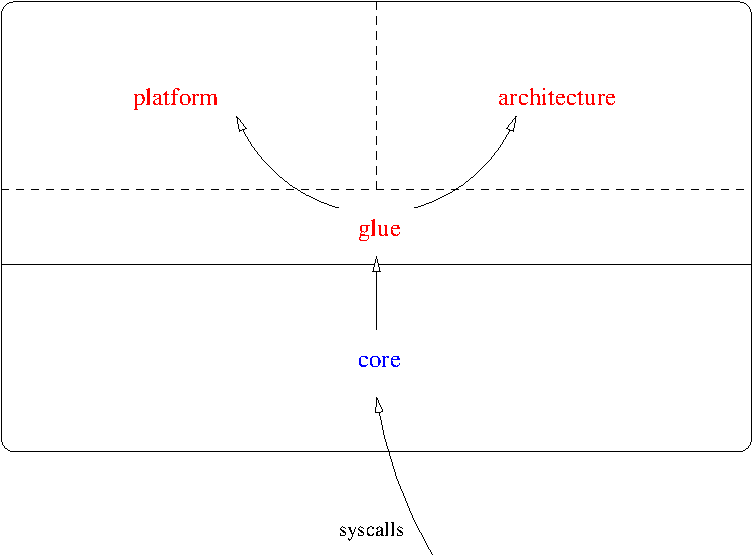
\includegraphics[scale=0.7]{\path/figures/kernel-layers.pdf}
    \caption{kaneton layers.}
    \label{figure:kernel-layers}
  \end{center}
\end{figure}

\textit{Figure \ref{figure:kernel-layers}} illustrates this decomposition where
system calls are first processed by the core which then calls the glue
component. This component knows how to handle operations depending on the
current couple platform/architecture. It then re-distribute the calls to
either the platform or architecture component.
